% mainDoc.tex - Main part of the document

\nonumsection*{ABSTRACT}\addcontentsline{toc}{section}{ABSTRACT}

Arrowtooth Flounder (\emph{Atheresthes stomias}, Turbot) is an important component of the trawl fishery in British Columbia.
See figure~\ref{fig:cpue} for cpue.

% \newpage	%French abstract must appear on new page

% \section*{R\'esum\'e}\addcontentsline{toc}{section}{R\'ESUM\'E}
\nonumsection*{R\'ESUM\'E}\addcontentsline{toc}{section}{R\'ESUM\'E}

% \addcontentsline{toc}{section}{R\'ESUM\'E}

\clearpage

% Need numbering back to Arabic.
\pagenumbering{arabic}
\setcounter{page}{1}

\section{INTRODUCTION}

This stock assessment is for Arrowtooth Flounder in combined Pacific Marine Fisheries Commission (PMFC) major areas 3C, 3D, 5A, 5B, 5C, 5D, and 5E off the west coast of British Columbia (Figure~\ref{fig:areas}). Arrowtooth Flounder make up a large component of the trawl fishery, but most are and have been discarded at sea. Proteolysis occurs in the muscle tissue of this species a short time after it is caught, which makes the flesh very mushy and unpalatable. There is a market in Korea for the frills, and a market for the fillets if they are frozen at sea, very shortly after capture.

CHANGE: Some background information is taken from  CHANGECITE: \citet{arf1995}, \citet{arf1999a}, \citet{arf1999b}, \citet{arf2000}, \citet{arf2001}, \citet{arf2003}, \citet{arf2006},\citet{arf2013}.

\subsection{BIOLOGICAL BACKGROUND}

Arrowtooth Flounder (\emph{Atheresthes stomias}, Turbot) is a species of flatfish found along the rim of the Northeast Pacific Ocean. The most distinguishing feature of Arrowtooth Flounder is its large teeth, for which it was named. As juveniles (<380mm), Arrowtooth Flounder are monomorphic. Arrowtooth Flounder are sexually dimorphic, with adult females being larger than males (Figure~\ref{fig:agelength}).

The life history of POP follows similar patterns to other \emph{Sebastes} species, with release of larvae that spend periods ranging from about three to twelve months as free-swimming pelagic larvae before settling to the bottom as juveniles. Reproduction appears to follow onshore-offshore migration patterns where females move onshore for insemination and then migrate deeper to the entrances of submarine gullies where they release larvae from February to May  larvae depend on vertical upwelling to bring them into the upper pelagic zone to facilitate growth and dispersal. The larvae can spend up to a year in the water column before settling on benthic habitat . Juvenile benthic habitat is shallow (100-200~m), compared to the depths occupied by adult POP, and comprises either rough rocky bottoms or high relief features such as boulders, anemones, sponges, and corals  maximum known age appears to be 103~y for a female specimen from Moresby Gully at 364~m in 2002, from the Department of Fisheries and Oceans Canada (DFO) Groundfish database GFBio.

\subsection{RANGE AND DISTRIBUTION}

Pacific Ocean Perch occur along the North Pacific rim, ranging from Honshu (Japan), through the Bering Sea, along the Aleutian Islands (Alaska), then southward through BC down to central Baja California. They appear to be most abundant north of 50$^\circ$~N . In BC (Figure~\ref{fig:cpue}), hotspots ($\geq$ the 0.95 quantile of catch per unit effort (CPUE) from trawl tows from 1996-2012) occur southeast of Moresby Island (Moresby Gully), southwest of Moresby Island (Anthony Island), northwest of Graham Island (Langara Spit), and in Dixon Entrance north of Graham Island; catch rates are relatively low in PMFC areas 3C and 3D, off the west coast of Vancouver Island. Pacific Ocean Perch has been encountered by the BC trawl fleet over an estimated 46,240~km$^2$ (Figure~\ref{fig:cpue}). For PMFC areas 3C and 3D, 98\% of the commercial captures of POP lie between depths 128~m and 581~m (Appendix~H).

\subsection{OVERVIEW OF FISHERY}

Pacific Ocean Perch supports the largest rockfish fishery in British Columbia (BC) with an annual coastwide TAC (total allowable catch) of 5,448~t in 2010, which is being progressively reduced to 5,189~t over three years (see Appendix~B). The mean annual coastwide catch was about 5,000~t from 2006-2010 and the mean coastwide landed value of the POP catch for 2007-2010 was \$4.4~million (landed value data from D.~Lau, DFO Economics Sector). The trawl fishery accounts for 99.98\% of the coastwide TAC, with the rest allocated to the hook and line fishery. A detailed history of the POP fishery prior to the inception of the observer trawl program in 1996 can be found in  

\section{ASSESSMENT BOUNDARIES AND BACKGROUND}

For this assessment, we use PMFC major areas 3C and 3D (herein referred to as area 3CD), covering most of the west coast of Vancouver Island (Figure~\ref{fig:areas}). The PMFC areas are similar but not identical to the groundfish management areas (GMAs) used by the DFO Groundfish Management Unit (GMU); those areas (Figure~\ref{fig:areas}) are more attuned to the pattern of fishing for a range of demersal species. We have not used the GMAs because reporting from these areas has only been available since 1996 and there is no procedure to alter historical landings to conform to current boundaries. The TAC for GMA 3CD has been 530~t since 1998. The mean catch from 2007-2011 in PMFC area 3CD was 547~t.

This is the first quantitative stock assessment for the stock of POP in area \area. The most recent POP assessment for BC waters considered only Queen Charlotte Sound (QCS, combined PMFC area 5ABC,  primary fishing grounds for POP. Previous population modelling for POP focused on Goose Island Gully, one of the three main gullies in QCS. extended their results to the rest of the BC coast. % based on CPUE analysis. 

% ******AE: edit numbers for 5DE, last sentence here into Abstract:

We follow several recent west coast Canadian rockfish assessments , in using a modified version of the Coleraine statistical catch-at-age software  Awatea, to implement the model (Appendix~F). The model is an annual two-sex catch-at-age model tuned to: three fishery-independent trawl survey series, annual estimates of commercial catch since 1940, and age composition data from the commercial fishery (15 years of data) and from one survey series (four years of data). 

The model estimates parameters from the stock-recruitment function, natural mortality (independently for females and males), catchability coefficients for the three survey series, and selectivity parameters for the commercial fishery and the one survey series for which age data are available.

The model is used to estimate the past and present vulnerable biomass (the biomass that is vulnerable to capture by the fishery, taking into account selectivity), spawning stock biomass (mature females only) and population age structure. Estimated parameters are then used to calculate maximum sustainable yield (MSY) and reference points. Projections are performed to estimate future probabilities of the spawning biomass being greater than the reference points under a range of constant catch scenarios. All of these calculations are made in a Bayesian context to capture the uncertainty associated with parameter estimation. Uncertainty relative to some data sets is explored through sensitivity runs (Appendix~I).

Advice for managers was requested (see Appendix~A) to be guided by the DFO Sustainable Fisheries Framework, particularly the Fishery Decision-making Framework Incorporating the Precautionary Approach . Consequently, advice to managers is presented as a set of decision tables that provide probabilities of exceeding reference points for various years of projections across a range of constant catch scenarios. 

A DFO Technical Working Group provided valuable guidance with respect to many of the decisions that were made in the course of this work.

\section{CATCH DATA}
*Table with history of quota and catch from 1996-present

The preparation methods and the full catch history for this assessment are given in Appendix~B. Catches were estimated back to 1940. Poorly reported historical catches by foreign fleets were reconstructed based on sparse historical sampling data, and minor catches from other capture methods have been added to the totals. All available discard estimates were added to the catches, with estimates of historical discards based on current observed levels. The resulting time series of catch data that is used as model input is shown in Figure~\ref{fig:catchRecon-3CD}, and reaches a peak of 7,753~t in 1966 (during a period of intense fishing by foreign fleets) and a recent (2007-2011) average catch of 547~t. Catch data were only available for part of 2012, and so, for input to the model, the 2012 catch total was assumed to be the same as for 2011. Information about other species caught concurrently with POP commercial catches is presented in Appendix~H.

\section{FISHERIES MANAGEMENT}

Appendix~B summarises all management actions taken for POP (coastwide) since 1979. In particular, there has been a 100\% onboard observer program for the offshore trawl fleet since 1996, an Individual Vessel Quota for TAC trawl species in place since 1997, and a recent reduction in the combined GMA 5ABCD total allowable catch (from 4,188~t to 3,413~t, implemented progressively over three years).

\vspace{15mm}   % just to shift up the headings on this page

\section{OVER-HARVESTING EXPERIMENT}

In the 1980s, experimental over-harvesting of POP stocks was attempted in two regions along the BC coast  objectives of the experiments included (i)~ground-truthing trawl survey biomass estimates, (ii)~estimating fishing mortality, (iii)~validating ageing techniques by introducing a large negative anomaly in the age composition, (iv)~exploring stock-recruitment relationships, and (v)~involving industry in research and management.

The first experiment occurred off the WCVI where a specified overharvest was set (TAC~= 500~t) from 1980 to 1984 before returning to a level deemed sustainable at 300~t  experiment experienced no implementation problems and reporting by industry was deemed acceptable. The 3C TAC was subsequently reduced to 100~t in 1986 and remained low until 1993. 

The second overharvesting experiment occurred in the Langara Spit area of PMFC 5E off the WCHG region. This experiment differed from the WCVI one in that quotas were removed entirely in 1983 to allow five years of unrestricted fishing followed by five years of severely limited fishing. However, a scheduled closure set for 1988 did not occur because the harvesters and the region had become dependent on the higher harvest levels. Some of the fishers maintained that there was little or no evidence of over-exploitation, and misreporting of catch could not be controlled. Discussions involving harvesters, politicians, and DFO managers (excluding the original researchers) negotiated extensions of the fishery, but eventually the Langara Spit area was closed in 1993.

\section{SURVEY DESCRIPTIONS}

Three sets of fishery independent survey indices were used to track changes in the biomass of the \area~stock (Appendix~C):

1. the west coast Vancouver Island (WCVI) synoptic survey series, from 2004-2012 (even years only), referred to here as the `WCVI synoptic survey series';

2. the United States National Marine Fisheries Service (NMFS) Triennial survey series, covering seven years from 1980-2011, referred to here as the `NMFS Triennnial survey series';

3. a set of historic Research Vessel GB~Reed surveys off the WCVI, for the four years 1967-1970, referred to here as the `GB Reed survey series'.

The relative biomass survey indices are used as data in the model along with the associated relative error for each index value. See Appendix~C for justification of inclusion or exclusion of survey data.

Pre-1996 commercial catch and effort data were also investigated with the intent of creating CPUE-based abundance indices for use in the stock assessment model.  This approach was abandoned because it was felt that there were problems with the reliability of the data as well as questions as to the representative nature of the resulting indices, given the schooling behaviour of the species and the capacity of fishers to target these schools. Given the concern that the resulting indices would be hyperstable, they were not used in this assessment.


\section{BIOLOGICAL INFORMATION}

\subsection{BIOLOGICAL SAMPLES}

Commercial catches of rockfish by trawl gear have been sampled for age proportions since the 1960s. However, only POP otoliths aged using the `break and burn' method have been included in the age samples for this assessment because the earlier surface ageing method is known to be biased  with increasing age. Practically, this means that no usable age data were available for this assessment prior to 1982. Commercial fishery age samples were summarised for each quarter, with samples combined within a trip and weighted by the POP catch weight for the sampled trip. The quarterly samples were then scaled by the quarterly landed commercial catch weights to give annual proportions-at-age data (details are in Appendix~E; Table F.1 gives the years of data).

Survey age samples were only available from the WCVI synoptic survey series for even years from 2004 to 2010 (the 2012 samples have not yet been aged). These samples were scaled to represent the total survey in a manner similar to that used for the commercial samples (see Appendix~E).


\subsection{GROWTH PARAMETERS}

Growth parameters for both sexes were taken from the POP QCS assessment , which estimated parameters from biological samples collected from 1978 to 2009 by research surveys and from the commercial fishery (Appendix~D). Estimates of growth parameters were compared across the major assessment areas (3CD, 5ABC and 5DE) and across sample origins (research and commercial), and found to be consistent in all comparisons . Consequently, the same sex-specific growth parameters have been used for all three assessment areas, with sex-specific growth specified as a three-parameter von Bertalanffy model that estimates length-at-age. Weights-at-age, used to convert population numbers to biomass, were given by an allometric length-weight relationship. See Appendix~D for details. 

\subsection{MATURITY}

The maturity ogive was also taken from . Stage of maturity was determined macroscopically, partitioning the samples into one of seven maturity stages  the months of January to June. The analysis was restricted to this period because it is the period of maximum expected maturity  assigned to stages 1 or 2 were considered immature while those assigned to stages 3-7 were considered mature. Data representing staged and aged females (using the break and burn method) were pooled from all sampling sources and the observed proportion mature at each age was calculated, and a model fitted (see Appendix~D).

\subsection{NATURAL MORTALITY}

PAST ASSESSMENTS have assumed M.... etc.. cite Fargo Starr and Alaska center assessments. Very sensitive to assumptions in the model iscam.

Male and female natural mortalities were estimated as parameters of the model (see Appendix~F), using an informed prior based on the marginal posterior distributions from the QCS POP assessment , specifically a normal prior with mean 0.07 and standard deviation 0.007 for both sexes (see Appendix~F). The QCS assessment used a prior based on a POP assessment for the Gulf of Alaska , with mean 0.06 and standard deviation 0.006.

In recent assessments , model runs that fixed natural mortality were also used to provide the final advice to managers. However, because we were able to develop a prior based on Canadian POP data, and since the resulting Bayesian estimates of natural mortality and steepness (defined below) are uncorrelated (Appendix~G), only runs that estimate natural mortality are used in this assessment (as agreed upon by the Technical Working Group). Prior distributions for all estimated parameters are given in Table F.4.

\section{AGE-STRUCTURED MODEL}

We attempted a two-sex, age-structured stochastic model to reconstruct the population trajectory of Arrowtooth Flounder in area \area~from ....
*Reference Appendix for model outputs and sensitivities...

REASONS model was rejected.

1940 to the beginning of 2013. Ages were tracked from 1 to 30, with 30 being an accumulator age class. Although an accumulator age class of 60 was used in the QCS assessment , initial exploration runs for this assessment did not perform well using 60 for the accumulator age class. Better model performance was obtained using age 30, which is consistent with the earlier Goose Island Gully POP assessment by . 

The population at the beginning of the reconstruction was assumed to be in equilibrium with average recruitment and no fishing. Selectivities by sex for one of the surveys and the commercial fishery were estimated using three parameters describing a half-Gaussian function (that is set to 1 above a certain age). The model equations and implementation are described in Appendix~F.

The model was fit to the available data (three sets of survey indices, 15 annual proportions-at-age samples from the commercial fishery and four proportions-at-age samples from the WCVI synoptic survey series) by minimising a function which summed the negative log-likelihoods arising from each data set, the deviations from mean recruitment and the penalties stemming from the Bayesian priors. The minimised MPD (mode of the posterior distribution) `best fit' was used as the starting point for the Bayesian search across the joint posterior distributions of the parameters using the Monte Carlo Markov Chain (MCMC) procedure. 

The MCMC procedure was run for 10,000,000 iterations, sampling every 10,000th, to give 1,000 samples. These samples were used to estimate parameters and quantities of interest, including stock sizes and the probabilities of being above reference points.

Initial model fits to the data gave sensible and consistent results. Numerous sensitivity runs that systematically explored the effect of different components of the data on model results did not seem justified, given the small amount of available data when spread over the long period of stock reconstruction (particularly for the early years). Two sensitivity runs are presented in Appendix~I, one exploring possible systematic catch mis-reporting from 1987-1995 and the other dropping the early (1967-1970) GB Reed survey series. We did not explore ageing error. Such a sensitivity run was conducted for the Yellowmouth Rockfish assessment , with the conclusion that a full investigation of ageing error would require an independent dedicated analysis, which was beyond the capacity of the current assessment.


% FROM SWEAVE:
% **** Go through all for 5DE

\section{RESULTS}

MOVE TO APPENDIX FOR MODEL RESULTS

The base case model run had credible fits to the data, as demonstrated by visual examination of the MPD fits and the patterns of residuals (results in Appendix G). The MCMC results showed satisfactory convergence of the MCMC search process (Appendix G). Priors and marginal posteriors of the estimated parameters are also given in Appendix G, along with the values of the estimated parameters (Table \ref{tab:MCMCpar}). For example, natural mortality is estimated as having median (and 5-95\% credible interval) of 0.069~(0.060-0.079) for females and 0.072~(0.063-0.082) for males. Steepness is estimated to be 0.70~(0.48-0.91). The remaining MCMC results, of more general interest, are given here.

Figure \ref{fig:VBcatch} shows the MCMC results for the estimated vulnerable biomass, together with the reconstructed historical catches, and Figure \ref{fig:BVBnorm} shows the estimated medians of vulnerable and spawning (mature females only) biomass relative to their unfished values. (The full MCMC results for spawning biomass are included later in Figure \ref{fig:Bproj} regarding projections). These demonstrate a slight decline in biomass from 1940 to 1960 with the onset of fishing, followed by a very sharp decline in the 1960s due to heavy fishing (primarily by foreign fleets). After the cessation of foreign fishing, the biomass increased through the remainder of the 1970s. The biomass then declined through the 1980s until the mid-1990s, and has since increased, with median values of relative biomass now above the 1980 values.

Estimates of various quantities of interest are given in Table \ref{tab:MCMCderived}. In particular, the median (and 5-95\% credible interval) for $B_{2013}/B_0$, the ratio of current spawning biomass ($B_{2013}$) to the unfished equilibrium level ($B_0$), is 0.41~(0.19-0.68); thus 0.41 is the value for the final circle in Figure \ref{fig:BVBnorm}.
% (This ratio is sometimes known as depletion).

The estimated recruitments (age-1 fish, Figure \ref{fig:recruitsMCMC}) in part further explain the aforementioned stock trajectory. There was lower-than-average recruitment in the early 1970s, which may, together with increased catches, explain why the vulnerable biomass declined through the 1980s (note the approximate ten-year lag from recruitment to fish becoming fully selected by the commercial fishery). There are a number of year classes with approximately double the long-term average recruitment. This is unlike the patterns observed for the QCS area 5ABC stock (Figure 5 of  and the companion assessment for area 5DE , which both exhibited a dominant 1976 year class (age-1 recruits in 1977) that was approximately five times larger than the long-term average recruitment.    

Figure \ref{fig:exploitMCMC} shows the estimated exploitation rates (ratio of total catch to the vulnerable biomass in the middle of the year), which peaked in the mid-1960s due to the large foreign catches, and then peaked again (although not as high) in the early 1990s due to increased domestic exploitation. Exploitation rates have remained low since the mid-1990s, with $u_{2012}$, the exploitation rate for 2012, estimated to be 0.035~(0.018-0.077).

Estimates of further quantities of interest, such as absolute values of biomass (rather than relative values), are also given in Table \ref{tab:MCMCderived}, as well as quantities based on MSY, discussed below. 

\section{RECCOMENTDATIONS AND YIELD OPTIONS}
1. Recommend catch for yield with and without 2005 Catch data.
2. the unused proportion of the quota

\subsection{CURRENT STOCK LEVEL}

The estimated median MSY (with 5-95\% credible interval, tonnes) is 1,048~(700-1,509), compared to the mean catch over the last 5 years (2007-2011) of 547~t. The MSY is calculated as an equilibrium yield under constant average recruitment. 

The estimated ratio $B_{2013}/\Bmsy$ of spawning biomass (mature females only) at the start of 2013 ($B_{2013}$) to the equilibrium spawning biomass that will support the maximum sustainable yield ($\Bmsy$), is 1.53~(0.55-3.32). 

As noted above, $B_{2013}/B_0$, the ratio of current spawning biomass to the unfished equilibrium level, is 0.41~(0.19-0.68). The estimate of the ratio $\Bmsy / B_0$ is 0.27~(0.18-0.36).

\subsection{REFERENCE POINTS}

Decision tables are presented with respect to two sets of reference points as determined from consultation with N.~Davis (DFO Groundfish Management Unit, pers.~comm.); see below for rationale for the reference points. Each set is based on either $\Bmsy$ or $B_0$. Decision tables are also given with respect to additional reference points based on current biomass and $\umsy$. All reference points and the associated probabilities were derived from the posterior distributions of Bayesian output from the model.

As part of the Sustainable Fisheries Framework, suggested provisional reference points to guide management and to assess harvest in relation to sustainability. Because alternative reference points for Canadian west coast groundfish species have not been specified by policy, the suggested provisional DFO limit and upper stock reference points of $0.4 \Bmsy$ and $0.8 \Bmsy$ have been adopted here. These were the reference points used for the POP stock in QCS . Note that no modelling has been carried out to determine the suitability of these reference points for these stocks, nor have acceptable levels of risk been specified.

The zone below the limit reference point ($0.4 \Bmsy$) is termed the ``critical zone'' while the zone lying between the two reference points is termed the ``cautious zone''.  The region above the upper stock reference point ($0.8 \Bmsy$) is termed the ``healthy zone''.  $\Bmsy$ is also reported here as an additional reference point because it ``provides a useful basis for comparing stocks'' when conducting meta-analyses of assessment results. 

Figure \ref{fig:compBmsy} shows the distribution of $B_{2013}/\Bmsy$ relative to the DFO Precautionary Approach provisional reference points of $0.4 \Bmsy$ and $0.8 \Bmsy$. The stock is estimated to be currently above the critical zone with probability P$(B_{2013} > 0.4 \Bmsy) = 0.99$, and in the healthy zone with probability P$(B_{2013} > 0.8 \Bmsy) = 0.87$. For comparison, Figure \ref{fig:compBmsy} also shows the estimated status of the other two POP stocks, where the status for the 5ABC stock is based on a different year.

A second component of the provisional harvest rule of concerns the relationship of the exploitation rate relative to that associated with MSY under equilibrium conditions ($\umsy$). The rule specifies that the exploitation rate should be at or below $\umsy$ when the stock is in the healthy zone, it should be ramped down when in the cautious zone, and it should be kept to an absolute minimum when in the critical zone. Figure \ref{fig:snail} shows the exploitation rate in 2012 relative to that at $\umsy$ (red dot and vertical red line). The estimated ratio of $u_{2012}/\umsy$ is $0.38~(0.13-1.43)$. The probability that the current exploitation rate is below that associated with MSY is P$(u_{2012} < \umsy) = 0.89$.

% ***Last line into Abstract for 5DE.

The blue and grey circles in Figure \ref{fig:snail} show that, based on medians, the stock is estimated to have been in the healthy zone since the start of fishing. The median exploitation rate has been $>\umsy$ for a total of 18 years, the most recent being 1995.  

Other agencies and jurisdictions often use `proxy' reference points that are expressed in terms of $B_0$ rather than $\Bmsy$ (e.g. $\Bmsy$ is often poorly estimated as it is dependent on a consistent fishery. Therefore, the reference points of $0.2 B_0$ and $0.4 B_0$ are also presented here (see decision tables described below), as for the Yellowmouth Rockfish assessment . These reference points are the respective default values used in New Zealand as a `soft' limit (below which management action needs to be taken) and a `target' biomass for low productivity stocks (a mean around which the biomass is expected to vary).

\subsection{PROJECTION RESULTS AND DECISION TABLES}

Projections were made to evaluate the future behaviour of the population under different levels of constant catch, given the model assumptions.  The projections, starting with the biomass at the beginning of 2013, were made over a range of constant catch strategies (0-2,000~t in 200~t steps) for each of the \numMCMC~MCMC samples in the posterior. Future recruitments were generated through the stock-recruitment function using recruitment deviations drawn randomly from a lognormal distribution with zero mean and constant standard deviation (see Appendix F for full details). Projections were made for 10 years, as agreed upon with N.~Davis (pers.~comm.). This time frame was considered as long enough to satisfy the `long-term' requirement of the Request for Science Information and Advice (Appendix A), yet short enough for the projected recruitments to be mainly based on individuals spawned before 2013 (and hence already estimated by the model).

Resulting projections of spawning biomass are shown for selected catch strategies (Figure \ref{fig:Bproj}). These suggest, for example, that the median spawning biomass is projected to increase for a constant catch of 600~t, which is larger than the recent average catch. 

Decision tables give the probabilities of the spawning biomass exceeding the reference points in specified years, for various constant catch strategies, calculated as the proportion of MCMC samples for which the biomass exceeded the given reference point. Note that catches are held constant, without feedback control simulation. Consequently, there is no ramping down of fishing mortality if the stock reaches the cautious or critical zones.

Results for the three $\Bmsy$-based reference points are presented in Tables \ref{tab:LRP10}-\ref{tab:Bmsy10}. As an example of how to read the tables, the estimated probability that the stock is in the provisional healthy zone in 2017 under a constant catch strategy of 1,000~t is P$(B_{2017} > 0.8 \Bmsy)=0.82$ (`1000' row and `2017' column of Table \ref{tab:URP10}). Results for the two $B_0$-based reference points are given in Tables \ref{tab:B00.2.10yr} and \ref{tab:B00.4.10yr}. 

For a constant catch of 600~t, above the average recent catch of 547~t, the probabilities of the stock remaining above the critical zone, P$(B_{t} > 0.4 \Bmsy)$, or in the healthy zone, P$(B_{t} > 0.8 \Bmsy)$, essentially remain constant over the ten-year projections (`600' rows in Tables \ref{tab:LRP10} and \ref{tab:URP10}). However, note that the median of spawning biomass, $B_t$, is estimated to increase over this time (600~t catch strategy in Figure~\ref{fig:Bproj}).

The probabilities over time also essentially remain constant (for a catch of 600~t) for the reference point $0.2 B_0$, as shown by P$(B_{t} > 0.2 B_0)$ in Table \ref{tab:B00.2.10yr}. However, for $0.4 B_0$, the probabilities increase over the 10 years from P$(B_{2013} > 0.4 B_0)=0.52$ to P$(B_{2023} > 0.4 B_0)=0.67$, Table \ref{tab:B00.4.10yr}. 

Also given are two further tables of potential interest to management. Table \ref{tab:Bcurr.10yr} gives probabilities P$(B_t > B_{\currYear})$ for the projected spawning biomass to exceed the current spawning biomass. Table \ref{tab:umsy.10yr} gives probabilities P$(u_t > u_\mathrm{MSY})$ for the projected exploitation rate to exceed that at MSY.

The choice of which decision table to use depends on the current status of the stock, since the status will determine the objectives, which may be based on conservation, stock growth or fisheries catch. 

\vspace{10mm}     % fix to close up gap with Projection Results and Decision Tables subheading, since this subsection now fits on one page.
\section{GENERAL COMMENTS}

The picture presented from this assessment is of a slow-growing, low productivity stock that was depleted to less than $\Bmsy$ due to commercial fishing by foreign fleets from 1965 to 1976 (Figures~\ref{fig:BVBnorm} and \ref{fig:snail}). The heavy exploitation during this period was followed by reduced recruitment (Figure~\ref{fig:recruitsMCMC}). Since then there have been a number of recruitment events that were approximately double the long-term mean, the highest occurring in 1990 and 2000. The biomass appears to have increased since 1996-1997 (Figure~\ref{fig:BVBnorm}), coinciding with the commencement of the observer and Individual Vessel Quota programs.

Annual exploitation rates increased during the 1960s and peaked in 1966, but decreased steadily thereafter to a low point in 1977 (Figure \ref{fig:exploitMCMC}). After this, the Canadian fishery steadily ramped up exploitation until 1994, and then, once the observer and Individual Vessel Quota programs were initiated, the exploitation rates quickly settled down to reach a mean of 0.039 (mean of the 1997-2012 medians), with a current median of 0.035. This is around half the estimated median natural mortality rates of 0.069 (females) and 0.072 (males).

The spawning biomass (mature females only) at the beginning of 2013 is estimated to be 0.41~(0.19-0.68) of $B_0$ and 1.53~(0.55-3.32) of $\Bmsy$. Using the DFO Precautionary Approach provisional reference points of $0.4 \Bmsy$ and $0.8 \Bmsy$ to define zones, the stock is estimated to be currently above the critical zone with probability P$(B_{2013} > 0.4 \Bmsy) = 0.99$, and in the healthy zone with probability P$(B_{2013} > 0.8 \Bmsy) = 0.87$ (and thus in the intermediate cautious zone with probability $0.12$).


The decision tables provide guidance on the selection of short-term TAC recommendations and describe the range of possible future outcomes over the projection period at fixed levels of annual catch. The accuracy of the projections is predicated on the model being correct and assumes no management intervention in the time period covered by the tables.

Uncertainty in the estimated parameters and quantities is explicitly addressed using a Bayesian approach, but reflects only the specified model and weights assigned to the various data components.  Sensitivity runs provide some insight into model uncertainty.  However, the sensitivity runs presented here do not differ greatly from the base run.

We expect that the results from the several surveys initiated in the previous decade will continue to provide monitoring capability for POP. Catches in the commercial groundfish fisheries are very well recorded. These ongoing initiatives give confidence that this stock is currently well monitored and that corrective action can be taken if required.

% \clearpage   % to not have to redo Bibliography as things are shifted.

\section{FUTURE RESEARCH AND DATA REQUIREMENTS}

The following issues could be considered when planning future stock assessments and management evaluations for Pacific Ocean Perch:

1. Continue the suite of fishery-independent trawl surveys that have been established along the BC coast. This includes obtaining age and length composition samples, which will allow the estimation of survey-specific selectivity ogives.

2. Review and potentially improve the commercial sampling program for POP age composition with the goal of continuing the representative sampling of all fisheries that take significant amounts of POP.

3. Research how best to incorporate the uncertainty of ageing error into Canadian rockfish assessment models --  the Sclerochronology Laboratory at the Pacific Biological Station currently records uncertainty for each aged otolith.


\section{ACKNOWLEDGEMENTS}

We thank the members of the Arrowtooth Flounder Technical Working Group (Rowan Haigh, Kendra Holt, Rob Kronlund, Barry Ackerman, Greg Workman) for their valuable advice as this project progressed. We thank participants of the Regional Peer Review meeting for their comments at the meeting, and Rowan Haigh for chairing. We especially thank James Thorsen (NOAA) and Joanne Morgan (DFO) for their written reviews of the working paper. We also thank Steve Wichkowski and the members of the Sclerochronology Laboratory at the Pacific Biological Station for their processing of Arrowtooth Flounder otoliths. 

% \clearpage

\addcontentsline{toc}{section}{BIBLIOGRAPHY}
\bibliographystyle{resDoc}
\bibliography{../../all}

% Will use \cite{***} (or \citet etc.) as appropriate for
%  reference ***. Andy's system is that the reference is
%  given in the bib file as {abc12}, where a,b,c are the initials
%  of the authors, and 12 is the year. DFO12 etc. for DFO
%  documents, though be careful in case there are multiple
%  with the same name. (Maybe DFO12a etc., or something similar).
% If >6 authors then first 4 letters of the first author's name.

\clearpage

%% Need figure, though this one didn't save well as an .eps
%\begin{figure}[htp]
%\begin{center}
%\epsfxsize=6in
%\epsfbox{mainDoc/dummyFig.eps}
%%\epsfbox{gma.popymr.amend.eps}
%\end{center}
%\caption{DUMMY FIGURE FOR NOW**. Pacific Marine Fisheries Commission (PMFC) major areas (outlined in dark blue) compared with Groundfish Management Unit areas for POP (shaded). For reference, map indicates Queen Charlotte Sound (QCS) and Goose Island Gully (GIG). This assessment is for the stock in PMFC areas 3C and 3D (termed area 3CD).} % ***5DE
%\label{fig:areas}
%\end{figure}

\begin{figure}[htp]
\begin{center}
\includegraphics[width=6in,keepaspectratio=true]{cpueFigures/ARF-1996-2014-CPUE.eps}
\end{center}
\vspace{0mm}
% To get the grid size in km^2 for the caption:
% While in the gui for the map, type mean(xtcall(PBSmap)$pdata$area) for the map you currently have loaded.
\caption{Mean catch-per-unit-effort (CPUE, kg/h) of Arrowtooth Flounder in grid cells 0.1$^\circ$ longitude by 0.075$^\circ$ latitude (roughly 57.8~km$^2$). The shaded cells give an approximation of the area where Arrowtooth Flounder was encountered by fishing events from the groundfish trawl fishery from January 1, 1996 to October 7, 2014. Contours are 200 m and 1000 m isobaths. Red lines are PFMA area boundaries.}
\label{fig:cpue}
\end{figure}

% Figures from Sweave (this gets copied pretty much as is straight from our
%  Sweave output from our R package PBSawatea):

% \ymrfig{VBcatch}{Estimated vulnerable biomass (boxplots) and commercial catch (vertical bars), in tonnes, over time. Boxplots show the 2.5, 25, 50, 75 and 97.5 percentiles from the MCMC results. Catch is shown to compare its magnitude to the estimated vulnerable biomass.}

%\ymrfig{BVBnorm}{Changes in $B_t / B_0$ and $V_t / V_0$ (spawning and vulnerable biomass relative to unfished equilibrium levels) over time, shown as the medians of the MCMC posteriors.}

% \ymrfig{recruitsMCMC}{Marginal posterior distribution of recruitment in 1,000's of age-1 fish plotted over time. Boxplots show the 2.5, 25, 50, 75 and 97.5 percentiles from the MCMC results. Note that the first year for which there are age data is 1982, and the plus-age class is 30, such that there are no direct data concerning age-1 fish before 1953. Also, the final few years have no direct age data from which to estimate recruitment, because fish are not fully selected until age 11 by the commercial vessels or age 15 by the WCVI synoptic survey (using the MCMC median ages of full selectivity for commercial catch, $\mu_{4}$, and WCVI survey $\mu_{1}$, Table \ref{tab:MCMCpar}).}


% \ymrfig{exploitMCMC}{Marginal posterior distribution of exploitation rate plotted over time. Boxplots show the 2.5, 25, 50, 75 and 97.5 percentiles from the MCMC results.}

\begin{figure}[htp]
\begin{center}
\epsfxsize=6in
\epsfbox{mainDoc/CompBmsy-POP-(3CD,5ABC,5DE).eps}
\end{center}
\caption{Current status of the three Canadian POP stocks relative to the DFO Precautionary Approach provisional reference points of $0.4 \Bmsy$ and $0.8 \Bmsy$. The value of $B_t / \Bmsy$ is for $t=2013$ for 3CD (this assessment) and 5DE , and for $t=2011$ for area 5ABC (run `Estimate $M \& h$' from  show the 5, 25, 50, 75 and 95 percentiles from the MCMC results.}
\label{fig:compBmsy} 
\end{figure}

%\ymrfig{snail}{Phase plot through time of the medians of the ratios $B_t / B_\mathrm{MSY}$ (the spawning biomass in year $t$ relative to $B_\mathrm{MSY}$) and $u_t / u_\mathrm{MSY}$ (the exploitation rate in year $t$ relative to $u_\mathrm{MSY}$). Blue filled circle is the starting year (1940). Years then proceed from light grey through to dark grey with the final year (2012) as a filled red circle, and the red lines represent the 10\% and 90\% percentiles of the posterior distributions for the final year. Vertical grey lines indicate the Precautionary Approach provisional limit and upper stock reference points of 0.4$B_\mathrm{MSY}$ and 0.8$B_\mathrm{MSY}$, and horizontal grey line indicates $u_\mathrm{MSY}$.}


%\ymrfig{Bproj}{Projected biomass (t) under different constant catch strategies (t); boxplots show the 2.5, 25, 50, 75 and 97.5 percentiles from the MCMC results. For each of the \numMCMC~samples from the MCMC posterior, the model was run forward in time (red, with medians in black) with a constant catch, and recruitment was simulated from the stock-recruitment function with lognormal error (see equation \ref{Rteqn}). For reference, the average catch over the last 5 years (2007-2011) is 547~t.}

% Commenting out for WG meeting, plus not so useful for short 
%  projections. 
% \ymrfig{Rproj}{Projected recruitments (red) under different constant catch strategies (boxplots show the 2.5, 25, 50, 75 and 97.5 percentiles from the MCMC results; historical recruitments in black).}
% xx = apply(currentProj$R$'0', 2, max)

\clearpage

% From Sweave:

\begin{table}[tp]
\centering
\caption{\label{tab:MCMCderived} The 5th, 50th and 95th percentiles of MCMC-derived quantities from the \numMCMC~samples of the MCMC posterior. Definitions are: $B_0$ -- unfished equilibrium spawning biomass (mature females), $V_0$ -- unfished equilibrium vulnerable biomass (males and females), $B_{2013}$ -- spawning biomass at the start of $2013$, $V_{2013}$ -- vulnerable biomass in the middle of 2013, $u_{2012}$ -- exploitation rate (ratio of total catch to vulnerable biomass) in the middle of 2012, $u_\mathrm{max}$ -- maximum exploitation rate (calculated for each sample as the maximum exploitation rate from 1940-2012), $\Bmsy$ -- equilibrium spawning biomass at MSY (maximum sustainable yield), $u_\mathrm{MSY}$ -- equilibrium exploitation rate at MSY, $V_\mathrm{MSY}$ -- equilibrium vulnerable biomass at MSY. All biomass values (and MSY) are in tonnes. For reference, the average catch over the last 5 years (2007-2011) is 547~t.}
\begin{tabular}{lrrr} 
\hline
Value & \multicolumn{3}{c}{Percentile}\\
\cline{2-4}
 & 5\% & 50\% & 95\% \\
\hline 
 & & & \\
& \multicolumn{3}{c}{From model output}\\
$B_0$                  & 17,562 & 21,442 & 27,877 \\
$V_0$                  & 32,687 & 38,855 & 49,469 \\
$B_{2013}$             & 3,888 & 8,745 & 17,269 \\
$V_{2013}$             & 7,360 & 16,427 & 32,072 \\

$B_{2013} / B_0$       & 0.189 & 0.406 & 0.684 \\
$V_{2013} / V_0$     & 0.199 & 0.420 & 0.708 \\

$u_{2012}$             & 0.018 & 0.035 & 0.077 \\
$u_\mathrm{max}$       & 0.221 & 0.288 & 0.418 \\
\hline
 & & & \\
& \multicolumn{3}{c}{MSY-based quantities}\\
$0.4 B_\mathrm{MSY}$   &  1,433 & 2,324 & 3,592 \\
$0.8 B_\mathrm{MSY}$   &  2,866 & 4,647 & 7,183 \\
$B_\mathrm{MSY}$       &  3,583 & 5,809 & 8,979 \\
$B_\mathrm{MSY} / B_0$ &  0.178 & 0.272 & 0.357 \\
$B_{2013} / B_\mathrm{MSY}$ & 0.552 & 1.526 & 3.323 \\

$\mathrm{MSY}$                    & 700 & 1,048 & 1,509 \\
$u_\mathrm{MSY}$       & 0.045 & 0.091 & 0.174 \\
$u_{2012} / u_\mathrm{MSY}$ & 0.134 & 0.384 & 1.434 \\

$V_\mathrm{MSY}$       & 7,586 & 11,729 & 17,112 \\
$V_\mathrm{MSY} / V_0$ & 0.213 & 0.301 & 0.379 \\
\hline
\end{tabular}	
\end{table}

\clearpage

% For Decision table write up **** add something like this to the header:
% Five-years:
% \multicolumn{7}{l}{P$(B_t > 0.4 \Bmsy)$} \\
%  \hline
%Annual catch & \multicolumn{6}{c}{Projection year} \\
%\cline{2-7}
%strategy & 2011 & 2012 & 2013 & 2014 & 2015 & 2016 \\

% 10-years:
% \multicolumn{12}{l}{P$(B_t > 0.4 \Bmsy)$} \\
% \hline
% Annual catch & \multicolumn{11}{c}{Projection year} \\
% \cline{2-12}
% strategy 

% latex table generated in R 2.15.0 by xtable 1.7-0 package
% Tue Oct 16 14:05:51 2012
\begin{table}[tbp]
\begin{center}
\caption{Decision table concerning the limit reference point $0.4 \Bmsy$ for 1-10 year projections for a range of constant catch strategies (in tonnes). Values are P$(B_t > 0.4 \Bmsy)$, i.e.~the probability of the spawning biomass (mature females) at the start of year $t$ being greater than the limit reference point. The probabilities are the proportion (to two decimal places) of the 1000 MCMC samples for which $B_t > 0.4 \Bmsy$. For reference, the average catch over the last 5 years (2007-2011) is 547~t.}
\label{tab:LRP10}
\begin{tabular}{rrrrrrrrrrrr}
\multicolumn{12}{l}{P$(B_t > 0.4 \Bmsy)$} \\
\hline
Annual catch & \multicolumn{11}{c}{Projection year} \\
\cline{2-12}
strategy & 2013 & 2014 & 2015 & 2016 & 2017 & 2018 & 2019 & 2020 & 2021 & 2022 & 2023 \\ 
  \hline
0 & 0.99 & 0.99 & 0.99 & 0.99 & 0.99 & 0.99 & 0.99 & 0.99 & 1.00 & 1.00 & 1.00 \\ 
  200 & 0.99 & 0.99 & 0.99 & 0.99 & 0.99 & 0.99 & 0.99 & 0.99 & 0.99 & 0.99 & 0.99 \\ 
  400 & 0.99 & 0.99 & 0.98 & 0.98 & 0.98 & 0.98 & 0.99 & 0.99 & 0.99 & 0.99 & 0.99 \\ 
  600 & 0.99 & 0.98 & 0.98 & 0.98 & 0.98 & 0.98 & 0.98 & 0.98 & 0.97 & 0.97 & 0.97 \\ 
  800 & 0.99 & 0.98 & 0.98 & 0.97 & 0.97 & 0.96 & 0.96 & 0.96 & 0.95 & 0.95 & 0.95 \\ 
  1000 & 0.99 & 0.98 & 0.97 & 0.96 & 0.95 & 0.95 & 0.94 & 0.94 & 0.93 & 0.93 & 0.92 \\ 
  1200 & 0.99 & 0.98 & 0.97 & 0.95 & 0.94 & 0.93 & 0.92 & 0.92 & 0.90 & 0.90 & 0.89 \\ 
  1400 & 0.99 & 0.98 & 0.95 & 0.94 & 0.92 & 0.92 & 0.90 & 0.88 & 0.87 & 0.84 & 0.83 \\ 
  1600 & 0.99 & 0.97 & 0.95 & 0.93 & 0.91 & 0.89 & 0.86 & 0.83 & 0.81 & 0.79 & 0.77 \\ 
  1800 & 0.99 & 0.97 & 0.94 & 0.92 & 0.89 & 0.85 & 0.82 & 0.79 & 0.76 & 0.74 & 0.72 \\ 
  2000 & 0.99 & 0.96 & 0.94 & 0.90 & 0.86 & 0.81 & 0.78 & 0.75 & 0.72 & 0.69 & 0.65 \\ 
   \hline
\end{tabular}
\end{center}
\end{table}% latex table generated in R 2.15.0 by xtable 1.7-0 package
% Tue Oct 16 14:05:51 2012
\begin{table}[tpb]
\begin{center}
\caption{Decision table for the upper reference point $0.8 \Bmsy$ for 1-10 year projections, such that values are P$(B_t > 0.8 \Bmsy)$. For reference, the average catch over the last 5 years (2007-2011) is 547~t.}
\label{tab:URP10}
\begin{tabular}{rrrrrrrrrrrr}
\multicolumn{12}{l}{P$(B_t > 0.8 \Bmsy)$} \\
\hline
Annual catch & \multicolumn{11}{c}{Projection year} \\
\cline{2-12}
strategy & 2013 & 2014 & 2015 & 2016 & 2017 & 2018 & 2019 & 2020 & 2021 & 2022 & 2023 \\ 
  \hline
0 & 0.87 & 0.88 & 0.90 & 0.92 & 0.93 & 0.94 & 0.94 & 0.95 & 0.96 & 0.96 & 0.97 \\ 
  200 & 0.87 & 0.88 & 0.89 & 0.90 & 0.91 & 0.92 & 0.93 & 0.93 & 0.94 & 0.95 & 0.95 \\ 
  400 & 0.87 & 0.87 & 0.88 & 0.88 & 0.89 & 0.90 & 0.91 & 0.91 & 0.92 & 0.92 & 0.93 \\ 
  600 & 0.87 & 0.86 & 0.86 & 0.86 & 0.87 & 0.87 & 0.88 & 0.88 & 0.88 & 0.88 & 0.89 \\ 
  800 & 0.87 & 0.86 & 0.85 & 0.84 & 0.85 & 0.85 & 0.85 & 0.84 & 0.85 & 0.85 & 0.85 \\ 
  1000 & 0.87 & 0.85 & 0.83 & 0.83 & 0.82 & 0.81 & 0.81 & 0.81 & 0.80 & 0.80 & 0.79 \\ 
  1200 & 0.87 & 0.84 & 0.82 & 0.81 & 0.79 & 0.78 & 0.77 & 0.76 & 0.75 & 0.74 & 0.72 \\ 
  1400 & 0.87 & 0.84 & 0.81 & 0.79 & 0.76 & 0.75 & 0.73 & 0.72 & 0.70 & 0.69 & 0.67 \\ 
  1600 & 0.87 & 0.83 & 0.80 & 0.76 & 0.74 & 0.71 & 0.69 & 0.67 & 0.65 & 0.63 & 0.61 \\ 
  1800 & 0.87 & 0.83 & 0.78 & 0.74 & 0.71 & 0.68 & 0.64 & 0.61 & 0.59 & 0.57 & 0.53 \\ 
  2000 & 0.87 & 0.82 & 0.77 & 0.72 & 0.68 & 0.63 & 0.60 & 0.57 & 0.53 & 0.49 & 0.46 \\ 
   \hline
\end{tabular}
\end{center}
\end{table}% latex table generated in R 2.15.0 by xtable 1.7-0 package
% Tue Oct 16 14:05:51 2012
\begin{table}[tbp]
\begin{center}
\caption{Decision table for the reference point $\Bmsy$ for 1-10 year projections, such that values are P$(B_t > \Bmsy)$. For reference, the average catch over the last 5 years (2007-2011) is 547~t.}
\label{tab:Bmsy10}
\begin{tabular}{rrrrrrrrrrrr}
\multicolumn{12}{l}{P$(B_t > \Bmsy)$} \\
\hline
Annual catch & \multicolumn{11}{c}{Projection year} \\
\cline{2-12}
strategy & 2013 & 2014 & 2015 & 2016 & 2017 & 2018 & 2019 & 2020 & 2021 & 2022 & 2023 \\ 
  \hline
0 & 0.78 & 0.80 & 0.82 & 0.84 & 0.86 & 0.88 & 0.90 & 0.91 & 0.92 & 0.93 & 0.94 \\ 
  200 & 0.78 & 0.80 & 0.81 & 0.82 & 0.84 & 0.85 & 0.87 & 0.88 & 0.89 & 0.90 & 0.91 \\ 
  400 & 0.78 & 0.79 & 0.80 & 0.80 & 0.81 & 0.82 & 0.84 & 0.85 & 0.85 & 0.86 & 0.87 \\ 
  600 & 0.78 & 0.78 & 0.79 & 0.78 & 0.79 & 0.79 & 0.80 & 0.81 & 0.82 & 0.82 & 0.83 \\ 
  800 & 0.78 & 0.77 & 0.77 & 0.76 & 0.76 & 0.76 & 0.76 & 0.77 & 0.77 & 0.77 & 0.77 \\ 
  1000 & 0.78 & 0.77 & 0.75 & 0.74 & 0.73 & 0.73 & 0.73 & 0.72 & 0.72 & 0.71 & 0.72 \\ 
  1200 & 0.78 & 0.76 & 0.74 & 0.71 & 0.70 & 0.69 & 0.68 & 0.68 & 0.67 & 0.67 & 0.66 \\ 
  1400 & 0.78 & 0.75 & 0.71 & 0.70 & 0.67 & 0.66 & 0.64 & 0.63 & 0.62 & 0.61 & 0.58 \\ 
  1600 & 0.78 & 0.74 & 0.70 & 0.66 & 0.64 & 0.61 & 0.60 & 0.58 & 0.56 & 0.54 & 0.52 \\ 
  1800 & 0.78 & 0.73 & 0.69 & 0.64 & 0.60 & 0.57 & 0.54 & 0.52 & 0.49 & 0.47 & 0.44 \\ 
  2000 & 0.78 & 0.72 & 0.66 & 0.61 & 0.56 & 0.53 & 0.49 & 0.46 & 0.44 & 0.40 & 0.37 \\ 
   \hline
\end{tabular}
\end{center}
\end{table}% latex table generated in R 2.15.0 by xtable 1.7-0 package
% Tue Oct 16 14:05:51 2012
\begin{table}[tbp]
\begin{center}
\caption{Decision table for the alternative reference point $0.2 B_0$ for 1-10 year projections, such that values are P$(B_t > 0.2 B_0)$. For reference, the average catch over the last 5 years (2007-2011) is 547~t.}
\label{tab:B00.2.10yr}
\begin{tabular}{rrrrrrrrrrrr}
\multicolumn{12}{l}{P$(B_t > 0.2 B_0)$} \\
\hline
Annual catch & \multicolumn{11}{c}{Projection year} \\
\cline{2-12}
strategy & 2013 & 2014 & 2015 & 2016 & 2017 & 2018 & 2019 & 2020 & 2021 & 2022 & 2023 \\ 
  \hline
0 & 0.94 & 0.95 & 0.96 & 0.97 & 0.97 & 0.98 & 0.98 & 0.99 & 0.99 & 0.99 & 0.99 \\ 
  200 & 0.94 & 0.94 & 0.95 & 0.96 & 0.96 & 0.97 & 0.97 & 0.98 & 0.98 & 0.98 & 0.98 \\ 
  400 & 0.94 & 0.94 & 0.94 & 0.95 & 0.95 & 0.95 & 0.96 & 0.96 & 0.96 & 0.96 & 0.96 \\ 
  600 & 0.94 & 0.94 & 0.94 & 0.93 & 0.93 & 0.93 & 0.93 & 0.94 & 0.94 & 0.94 & 0.94 \\ 
  800 & 0.94 & 0.94 & 0.93 & 0.91 & 0.91 & 0.90 & 0.91 & 0.90 & 0.90 & 0.90 & 0.89 \\ 
  1000 & 0.94 & 0.93 & 0.91 & 0.89 & 0.89 & 0.88 & 0.87 & 0.86 & 0.86 & 0.85 & 0.84 \\ 
  1200 & 0.94 & 0.92 & 0.90 & 0.88 & 0.85 & 0.84 & 0.83 & 0.81 & 0.80 & 0.79 & 0.78 \\ 
  1400 & 0.94 & 0.91 & 0.88 & 0.85 & 0.82 & 0.79 & 0.78 & 0.76 & 0.74 & 0.73 & 0.72 \\ 
  1600 & 0.94 & 0.90 & 0.86 & 0.82 & 0.78 & 0.75 & 0.74 & 0.72 & 0.69 & 0.66 & 0.64 \\ 
  1800 & 0.94 & 0.90 & 0.84 & 0.79 & 0.76 & 0.72 & 0.69 & 0.65 & 0.62 & 0.59 & 0.57 \\ 
  2000 & 0.94 & 0.89 & 0.82 & 0.77 & 0.72 & 0.68 & 0.64 & 0.59 & 0.57 & 0.52 & 0.48 \\ 
   \hline
\end{tabular}
\end{center}
\end{table}% latex table generated in R 2.15.0 by xtable 1.7-0 package
% Tue Oct 16 14:05:51 2012
\begin{table}[tbp]
\begin{center}
\caption{Decision table for the alternative reference point $0.4 B_0$ for 1-10 year projections, such that values are P$(B_t > 0.4 B_0)$. For reference, the average catch over the last 5 years (2007-2011) is 547~t.}
\label{tab:B00.4.10yr}
\begin{tabular}{rrrrrrrrrrrr}
\multicolumn{12}{l}{P$(B_t > 0.4 B_0)$} \\
\hline
Annual catch & \multicolumn{11}{c}{Projection year} \\
\cline{2-12}
strategy & 2013 & 2014 & 2015 & 2016 & 2017 & 2018 & 2019 & 2020 & 2021 & 2022 & 2023 \\ 
  \hline
0 & 0.52 & 0.57 & 0.62 & 0.67 & 0.70 & 0.74 & 0.78 & 0.81 & 0.84 & 0.86 & 0.87 \\ 
  200 & 0.52 & 0.56 & 0.59 & 0.64 & 0.67 & 0.70 & 0.73 & 0.75 & 0.77 & 0.80 & 0.81 \\ 
  400 & 0.52 & 0.54 & 0.56 & 0.59 & 0.62 & 0.66 & 0.68 & 0.70 & 0.71 & 0.73 & 0.75 \\ 
  600 & 0.52 & 0.52 & 0.53 & 0.55 & 0.58 & 0.60 & 0.63 & 0.64 & 0.65 & 0.66 & 0.67 \\ 
  800 & 0.52 & 0.51 & 0.51 & 0.51 & 0.52 & 0.55 & 0.56 & 0.57 & 0.59 & 0.59 & 0.60 \\ 
  1000 & 0.52 & 0.50 & 0.49 & 0.48 & 0.48 & 0.49 & 0.50 & 0.51 & 0.52 & 0.51 & 0.51 \\ 
  1200 & 0.52 & 0.49 & 0.46 & 0.44 & 0.44 & 0.44 & 0.45 & 0.44 & 0.44 & 0.43 & 0.42 \\ 
  1400 & 0.52 & 0.48 & 0.44 & 0.42 & 0.40 & 0.38 & 0.38 & 0.38 & 0.37 & 0.35 & 0.33 \\ 
  1600 & 0.52 & 0.47 & 0.42 & 0.40 & 0.36 & 0.35 & 0.32 & 0.31 & 0.30 & 0.28 & 0.27 \\ 
  1800 & 0.52 & 0.46 & 0.40 & 0.36 & 0.33 & 0.30 & 0.28 & 0.26 & 0.25 & 0.24 & 0.22 \\ 
  2000 & 0.52 & 0.44 & 0.38 & 0.34 & 0.29 & 0.27 & 0.23 & 0.21 & 0.20 & 0.18 & 0.16 \\ 
   \hline
\end{tabular}
\end{center}
\end{table}


% latex table generated in R 2.15.0 by xtable 1.7-0 package
% Wed Feb 20 16:16:31 2013
\begin{table}[ht]
\begin{center}
\caption{Decision table for comparing the projected biomass to the current biomass, given by probabilities P$(B_t > B_{\currYear})$. For reference, the average catch over the last 5 years (2007-2011) is 547~t.}
\label{tab:Bcurr.10yr}
\begin{tabular}{rrrrrrrrrrrr}
\multicolumn{12}{l}{P$(B_t > B_{\currYear})$} \\
  \hline
 & 2013 & 2014 & 2015 & 2016 & 2017 & 2018 & 2019 & 2020 & 2021 & 2022 & 2023 \\ 
  \hline
0 & -~ & 0.99 & 0.99 & 0.99 & 0.99 & 0.98 & 0.98 & 0.99 & 0.99 & 0.99 & 0.99 \\ 
  200 & -~ & 0.95 & 0.93 & 0.93 & 0.93 & 0.93 & 0.93 & 0.94 & 0.94 & 0.94 & 0.94 \\ 
  400 & -~ & 0.80 & 0.76 & 0.76 & 0.77 & 0.79 & 0.81 & 0.82 & 0.83 & 0.85 & 0.85 \\ 
  600 & -~ & 0.58 & 0.54 & 0.56 & 0.57 & 0.60 & 0.63 & 0.66 & 0.67 & 0.68 & 0.70 \\ 
  800 & -~ & 0.39 & 0.37 & 0.38 & 0.42 & 0.44 & 0.47 & 0.50 & 0.52 & 0.53 & 0.53 \\ 
  1000 & -~ & 0.24 & 0.24 & 0.26 & 0.29 & 0.32 & 0.34 & 0.36 & 0.38 & 0.38 & 0.38 \\ 
  1200 & -~ & 0.16 & 0.16 & 0.17 & 0.20 & 0.22 & 0.25 & 0.26 & 0.26 & 0.27 & 0.27 \\ 
  1400 & -~ & 0.10 & 0.10 & 0.12 & 0.14 & 0.16 & 0.17 & 0.18 & 0.19 & 0.19 & 0.19 \\ 
  1600 & -~ & 0.06 & 0.07 & 0.08 & 0.10 & 0.11 & 0.12 & 0.12 & 0.13 & 0.13 & 0.13 \\ 
  1800 & -~ & 0.04 & 0.04 & 0.06 & 0.07 & 0.08 & 0.09 & 0.09 & 0.09 & 0.09 & 0.09 \\ 
  2000 & -~ & 0.03 & 0.03 & 0.03 & 0.04 & 0.05 & 0.06 & 0.07 & 0.07 & 0.07 & 0.06 \\ 
   \hline
\end{tabular}
\end{center}
\end{table}


% latex table generated in R 2.15.0 by xtable 1.7-0 package
% Wed Feb 20 16:16:31 2013
\begin{table}[ht]
\begin{center}
\caption{Decision table for comparing the projected exploitation rate to that at MSY, such that values are P$(u_t > u_\mathrm{MSY})$, i.e.~the probability of the exploitation rate in the middle of year $t$ being greater than that at MSY. For reference, the average catch over the last 5 years (2007-2011) is 547~t.}
\label{tab:umsy.10yr}
\begin{tabular}{rrrrrrrrrrrr}
\multicolumn{12}{l}{P$(u_t > u_\mathrm{MSY})$} \\
  \hline
       & 2013 & 2014 & 2015 & 2016 & 2017 & 2018 & 2019 & 2020 & 2021 & 2022 & 2023 \\ 
  \hline
     0 & 0.00 & 0.00 & 0.00 & 0.00 & 0.00 & 0.00 & 0.00 & 0.00 & 0.00 & 0.00 & 0.00 \\ 
   200 & 0.01 & 0.01 & 0.01 & 0.01 & 0.01 & 0.01 & 0.00 & 0.00 & 0.00 & 0.00 & 0.00 \\ 
   400 & 0.05 & 0.05 & 0.05 & 0.05 & 0.05 & 0.04 & 0.04 & 0.04 & 0.04 & 0.04 & 0.04 \\ 
   600 & 0.12 & 0.12 & 0.12 & 0.12 & 0.11 & 0.11 & 0.10 & 0.10 & 0.10 & 0.11 & 0.11 \\ 
   800 & 0.20 & 0.20 & 0.20 & 0.21 & 0.21 & 0.20 & 0.20 & 0.20 & 0.20 & 0.20 & 0.20 \\ 
  1000 & 0.28 & 0.29 & 0.30 & 0.31 & 0.31 & 0.31 & 0.30 & 0.30 & 0.31 & 0.31 & 0.31 \\ 
  1200 & 0.38 & 0.40 & 0.40 & 0.41 & 0.40 & 0.40 & 0.41 & 0.41 & 0.41 & 0.42 & 0.43 \\ 
  1400 & 0.46 & 0.48 & 0.49 & 0.51 & 0.52 & 0.52 & 0.52 & 0.53 & 0.54 & 0.55 & 0.57 \\ 
  1600 & 0.54 & 0.56 & 0.58 & 0.60 & 0.61 & 0.61 & 0.62 & 0.63 & 0.65 & 0.65 & 0.67 \\ 
  1800 & 0.60 & 0.63 & 0.65 & 0.67 & 0.68 & 0.70 & 0.70 & 0.72 & 0.72 & 0.74 & 0.75 \\ 
  2000 & 0.66 & 0.70 & 0.73 & 0.75 & 0.75 & 0.77 & 0.78 & 0.79 & 0.80 & 0.81 & 0.82 \\ 
   \hline
\end{tabular}
\end{center}
\end{table}

\clearpage
